\documentclass[a4paper,pdf]{article} % gebruik acm style voor je scriptie: [format=acmsmall, screen=true, review=false]{acmart} 
\usepackage{amsmath}
\usepackage{amsfonts}
\usepackage{amssymb}
\usepackage{hyperref}
\usepackage{pdfpages} % http://mirror.unl.edu/ctan/macros/latex/contrib/pdfpages/pdfpages.pdf
\usepackage{booktabs} 


\usepackage[utf8]{inputenc}
\usepackage{amsmath}
\usepackage{graphicx}
\usepackage[colorinlistoftodos]{todonotes} % handig voor commentaar: gebruik \todo{}, zie ftp://ftp.fu-berlin.de/tex/CTAN/macros/latex/contrib/todonotes/todonotes.pdf
\usepackage{listings}
\usepackage{pdfpages}
\usepackage{tcolorbox}
\usepackage{float}
\usepackage{caption}
\usepackage{subcaption}


% when writing in Dutch
%\usepackage[dutch]{babel}
%\selectlanguage{dutch}


% linenumbering  See https://texblog.org/2012/02/08/adding-line-numbers-to-documents/
\usepackage{lineno}
\linenumbers


\begin{document}




%\input{titlepage}
%\documentclass[]{article}
%\usepackage{lmodern}
%%\usepackage{fontspec}
%\usepackage{amssymb,amsmath}
%\usepackage{ifxetex,ifluatex}
%\usepackage{fixltx2e} % provides \textsubscript
%\ifnum 0\ifxetex 1\fi\ifluatex 1\fi=0 % if pdftex
%  \usepackage[T1]{fontenc}
%  \usepackage[utf8]{inputenc}
%\else % if luatex or xelatex
%  \ifxetex
%    \usepackage{mathspec}
%    \usepackage{xltxtra,xunicode}
%  \else
%    \usepackage{fontspec}
%  \fi
%  \defaultfontfeatures{Mapping=tex-text,Scale=MatchLowercase}
%  \newcommand{\euro}{€}
%\fi
%% use upquote if available, for straight quotes in verbatim environments
%\IfFileExists{upquote.sty}{\usepackage{upquote}}{}
%% use microtype if available
%\IfFileExists{microtype.sty}{%
%\usepackage{microtype}
%\UseMicrotypeSet[protrusion]{basicmath} % disable protrusion for tt fonts
%}{}
%\usepackage{graphicx}
%\makeatletter
%\def\maxwidth{\ifdim\Gin@nat@width>\linewidth\linewidth\else\Gin@nat@width\fi}
%\def\maxheight{\ifdim\Gin@nat@height>\textheight\textheight\else\Gin@nat@height\fi}
%\makeatother
%% Scale images if necessary, so that they will not overflow the page
%% margins by default, and it is still possible to overwrite the defaults
%% using explicit options in \includegraphics[width, height, ...]{}
%\setkeys{Gin}{width=\maxwidth,height=\maxheight,keepaspectratio}
%\ifxetex
%  \usepackage[setpagesize=false, % page size defined by xetex
%              unicode=false, % unicode breaks when used with xetex
%              xetex]{hyperref}
%\else
%  \usepackage[unicode=true]{hyperref}
%\fi
%\hypersetup{breaklinks=true,
%            bookmarks=true,
%            pdfauthor={},
%            pdftitle={},
%            colorlinks=true,
%            citecolor=blue,
%            urlcolor=blue,
%            linkcolor=magenta,
%            pdfborder={0 0 0}}
%\urlstyle{same}  % don't use monospace font for urls
%\setlength{\parindent}{0pt}
%\setlength{\parskip}{6pt plus 2pt minus 1pt}
%\setlength{\emergencystretch}{3em}  % prevent overfull lines
%\setcounter{secnumdepth}{0}
%
%\date{}
%
%\begin{document}


\begin{titlepage}


\begin{center}
 
\textsc{\Large   Ideologie en classificatie in de Handelingen van de Tweede Kamer}

\bigskip

\textsc{\large
submitted in partial fulfillment for the degree of bachelor of science\\
%
\bigskip
Jasper van der Heide\\
%
10732721\\
%
\bigskip
Bachelor Informatiekunde\\
%
Faculteit der Natuurwetenschappen, Wiskunde en Informatica\\
%
Universiteit van Amsterdam\\
%
\bigskip
2018-06-28
}

\end{center}
 

\vfill

% In case of an internal project, remove External Supervisor or if you had two internal supervisors, change the header into 
%  & First Supervisor & Second Supervisor  \\
\begin{center}
\begin{tabular}{|l||ll|}
\hline
 & \textbf{Begeleider} & \textbf{Tweede lezer}  \\   
 \hline
\textbf{Titel, Naam} & Dr Maarten Marx&  \\
\textbf{Affliatie} &UvA, FNWI, IvI & \\ 
\textbf{Email} & maartenmarx@uva.nl& . \\
\hline
\end{tabular}
\end{center}


\bigskip

% logos
\begin{center}
\mbox{
\includegraphics[width=.2\paperwidth]{logo-uva.png} 
%\includegraphics[width=.2\paperwidth]{TitlePages/logos/ads.png}

}
\end{center}
\end{titlepage}

%
%\newpage
%
%\end{document}
  % or use another template

\pagebreak

\todototoc
\listoftodos
\tableofcontents

\pagebreak

\begin{abstract}
% [CHANGE] 
\end{abstract}


\section*{Thesis requirements}
\begin{itemize}
\item Your thesis is written in ACM style with two columns  (\texttt{documentclass[sigconf]{acmart}}).
\item It is maximally 10 pages long, excluding the title page and the appendix, but including references, figures, etc
\end{itemize}


\pagebreak


% Here you input all your sections in seperate files

\section{Introduction}
\label{sec:intro}
Teksten van politieke partijen kunnen bruikbaar zijn voor het bepalen van ideologische positie van andere teksten, aangezien zij zowel een tekst leveren als ook een bekende ideologie. Deze informatie kan vervolgens toegepast worden bij andere teksten die wellicht ideologisch van aard zijn. Bijvoorbeeld, op basis van deze informatie kan men teksten uit kranten classificeren op basis van ideologie.\par
In diverse landen zijn al verschillende onderzoeken gedaan naar het classificeren van partij-affiliatie op basis van teksten van politici.\cite{Ferreira2016UsingTT} Mede omdat elk land een andere politiek stelsel en cultuur heeft, verschillen de resultaten. Daarnaast gebruikt elk onderzoek ook een andere methode voor het classificeren. \par
Een onderzoek gericht op het Nederlandse parlement ontbreekt hierbij nog. Daarnaast focust elk onderzoek tot nu toe op een beperkte aantal methoden, dus geen brede analyse van de mogelijke methoden. \par
Dit onderzoek richt zich daarom op een breder scala aan mogelijke methoden en daarnaast ook specifiek op de Nederlandse politiek. De onderzoeksvraag luidt daarom dus ook:"Wat is het beste classificatiemodel voor het classificeren van sprekers in de Tweede Kamer op basis van partij-affiliatie?"\par
In dit onderzoek zal eerst gekeken worden naar welke methoden gangbaar zijn in vergelijkbare onderzoeken, maar ook naar welke methoden nieuw en potentieel zijn. Deze worden vervolgens geëvalueerd en vergeleken, in de hoop hiermee de onderzoeksvraag te kunnen beantwoorden.


\paragraph{Overview of thesis}
In sectie 2 zullen vergelijkbare onderzoeken uit andere landen besproken worden. In sectie 3 zal vervolgens de wijze waarop de verschillende classificatiemethoden gebruikt zijn als ook geëvalueerd zijn besproken worden. In sectie 4 zullen vervolgens de resultaten weergegeven worden. In sectie 5 zullen dan een evaluatie plaatsvinden van zowel de resultaten als de gehanteerde methodologie. In sectie 6 wordt dan ten slotte de onderzoeksvraag beantwoord.

\section{Related Work}
\label{sec:rel}

Deze sectie bestaat uit een aantal "blokken", waarin je per blok de relevante literatuur beschrijft. 

Neem alleen literatuur op die van belang is voor jouw onderzoeksvraag en deelvragen.

Typisch heb je 1 blok voor je hoofdvraag en per deelvraag \textbf{RQi} een blok. 


\subsection{RQ1}

\subsection{RQ2}

\section{Methodologie}
\label{sec:meth}


\subsection{De data}
\label{data}
De data die gebruikt worden, zijn de Handelingen van de Tweede Kamer gedurende het missionaire kabinet-Rutte II (5 november 2012 tot 22 maart 2017). Er is gekozen voor dit kabinet, omdat de data hiervoor makkelijk verkrijgbaar was, het kabinet lang zat, waardoor er veel data is, en het recent is waardoor het makkelijker te interpreteren is. Deze data zijn in xml-formaat van de website officielebekendmakingen.nl gehaald, samen met corresponderende metadata xml-bestanden. De bestanden van de Handelingen bevatten voornamelijk informatie over spreekbeurten tijdens een debat, waaronder naam van een spreker, partij-affiliatie, inhoud van de spreekbeurt en het soort spreekbeurt. Deze gegevens zijn samengevoegd tot een tabel en opgeslagen als csv-bestand.\par
Deze dataset bestaat uit een aantal soorten spreekbeurten; debat bijdragen, interrupties en antwoorden. Debat bijdrage is de eerste onafgebroken spreekbeurt die een spreker geeft achter het spreekgestoelte, aangeduid in de xml-file met het attribuut \textit{nieuw="ja"}. Dit kan een bijdrage in een debat zijn of een vraag tijdens een vragenuur. Interrupties zijn de vragen die andere politici stellen vanachter de interruptiemicrofoon aan de spreker. De antwoorden zijn vervolgens de reactie van een spreker achter het spreekgestoelte op een interruptie. Aangezien een debat bijdrage geïnterrumpeerd kan worden, kan deze inhoudelijk doorlopen in een antwoord van een spreker. Er is in dit onderzoek ervoor gekozen om gebruik te maken van een debat bijdrage samengevoegd tot één document met alle bijbehorende antwoorden van die spreker. Daarnaast zijn er verschillende soorten sprekers; de voorzitter, Tweede Kamerleden, leden van het kabinet en gastsprekers.  Daarnaast is alleen gekozen voor sprekers waarvan er een partij-affiliatie vermeld staat, dit is niet het geval voor leden van het kabinet, de voorzitter en gastsprekers  (met uitzondering van Nederlandse leden van het Europees Parlement).\par
Deze dataset bevat vervolgens naast de verkozen partijen van de 2012 Tweede Kamerverkiezingen, ook afsplitsingen van die partijen (tien in totaal) en bezoeken van vertegenwoordigingen van Nederlandse partijen uit het Europees Parlement (tien in totaal). Omdat van beide categorieën relatief weinig data is en er overlap zit met hun oorspronkelijke partij, zijn deze er uit gehaald. \par

De documenten verschillen vervolgens in grootte. De distributie lijkt op een lognormale verdeling, maar met een Kolmogorov-Smirnov test is hier geen bewijs voor gevonden \cite{Scipy}.

\begin{figure}[H]
    \centering
    \hspace*{-1in}
    \subfloat[label 1]{{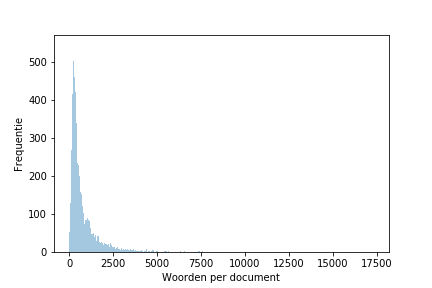
\includegraphics[width=9cm]{Verslag/Tables/lengthtexts.png} }}%
    \subfloat[label 2]{{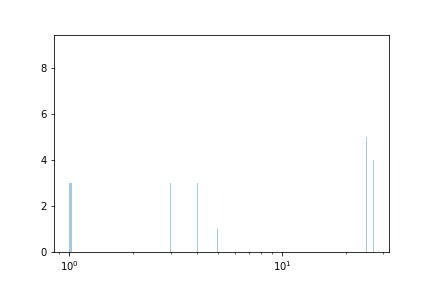
\includegraphics[width=9cm]{Verslag/Tables/lengthtextslog.png} }}%
    \caption{Aantal woorden per document}%
    \label{fig:example}%
\end{figure}
Om toch de uitschieters er uit te halen, is aangenomen dat het wel lognormaal verdeeld is en zijn daarmee de documenten buiten het betrouwbaarheidsinterval van 95\% eruit gehaald. De documenten met een lengte van minimaal 28 en maximaal 1492 woorden bleven daarmee over. Het gemiddelde is daarna 498 woorden en de mediaan is 386 woorden. Een totaal aantal documenten van 14899 blijven vervolgens over.\par

\begin{table}[H]
\label{aantallen}
\caption{Aantal documenten per partij gedurende het missionaire kabinet-Rutte II.}
\centering
\begin{tabular}{lrrr}
\toprule
{} &  Totaal &  Vragenuur &  Debat \\
\midrule
SP           &    2284 &        107 &   2177 \\
CDA          &    1901 &         88 &   1813 \\
D66          &    1889 &        133 &   1756 \\
PvdA         &    1821 &        112 &   1709 \\
PVV          &    1700 &         49 &   1651 \\
VVD          &    1694 &         76 &   1618 \\
ChristenUnie &    1068 &         32 &   1036 \\
GroenLinks   &    1068 &         47 &   1021 \\
SGP          &     655 &         10 &    645 \\
PvdD         &     432 &         14 &    418 \\
50PLUS       &     387 &         12 &    375 \\
\bottomrule
\end{tabular}

\end{table}
Deze 14899 documenten zijn verdeeld over 2984 debatten, waarbij elke vraag tijdens het vragenuur als één debat gezien wordt. Op basis van de aantallen is er voor classificatie een baseline nauwkeurigheid van 0.15 (door altijd grootste partij te kiezen) en baseline $F_1$ score van 0.11 (door willekeurig te voorspellen gewogen bij aantal spreekbeurten in klasse).\par


\subsection{Methoden}


\subsubsection{Deelvraag 1}
Om deze deelvraag te beantwoorden zullen een aantal classificatiemethoden vergeleken worden. Aangezien het onmogelijk is om alle classificatiemethoden te vergelijken, beperkt dit onderzoek zich tot classificatiemethoden die gebruikt zijn in vergelijkbare onderzoeken, zoals besproken in \ref{sec:Deelvraag1}. Er is ervoor gekozen om alleen gebruik te maken van methoden waarvan reeds implementaties beschikbaar waren in Python. Voor alle methoden wordt gezocht naar de beste parameters; een grid search. Deze grid search wordt gedaan door middel van 5-fold cross-validation, waarbij de trainings set steeds 80\% is en de test set 20\% van de totale dataset.

\paragraph{Pre-processing}
Voor pre-processing is gebruik gemaakt van tokenisation en lowercasing. Voor tokenisation is de reguliere expressie $\\w+$ gebruikt, die daarmee alleen de letters en cijfers overhoudt. Deze woorden zijn vervolgens allemaal omgezet in kleine letters. Vervolgens is er gevarieerd tussen wel of geen gebruik maken van stemming. In het geval van stemming is gebruik gemaakt van de Snowball Stemmer via de Python NLTK module.

\paragraph{Bag-of-words model}
Bag-of-words model is de meest gebruikte representatie van data in vergelijkbare onderzoeken. Bij het bag-of-words model wordt elk document gerepresenteerd door een vector, waarbij elke kolom een woord voorstelt met een bijbehorende waarde. Voornaamste beperking van dit model is dat het geen rekening houdt met de volgorde van woorden, wat een groot effect kan hebben op de betekenis van een document.\par
Voor dit onderzoek zijn de volgende wegingen voor woorden getest: \textit{boolean} (wel of niet aanwezig), \textit{tf} (woordfrequentie), \textit{tf-norm} (woordfrequentie genormaliseerd door documentlengte) en \textit{tf-idf}
Daarnaast wordt in dit onderzoek geëxperimenteerd met een minimale of maximale woord- of documentfrequentie. Ook is gekeken naar het effect van combinaties van n-grams; unigrams, bigrams en trigrams. N-grams zijn combinaties van N aantal opeenvolgende woorden. Bij een unigram is elke feature gewoon één woord, terwijl bij een bigram dit twee opvolgende woorden zijn. Dit kan nuttig zijn, want als bijvoorbeeld het woord \textit{asfalt} er in voorkomt, dan maakt het voor ideologie waarschijnlijk meer uit of er \textit{minder asfalt} of \textit{meer asfalt} staat.\par

\paragraph{Support Vector Machines en Logistische Regressie}
De meest voorkomende techniek in vergelijkbaar onderzoek is Support Vector Machine (SVM). Een andere techniek die gebruikt wordt is logistische regressie. Beide kennen een eigen implementatie in sklearn, maar deze implentaties zijn niet efficiënt met grote datasets. Om deze reden is er in beide gevallen voor gekozen om gebruik te maken van de functie SGDClassifier, die beide technieken leert met \textit{stochastic gradient descent learning}. Er is hiervoor gevarieerd met de regularisatie, learning rate en maximum aantal iteraties. Voor regularisatie is hier geëxperimenteerd met Lasso en Ridge regularisatie, en een combinatie van beide genaamd Elasticnet. De andere parameters zijn gelaten op de standaardwaarden van scikit-learn \cite{scikit-learn}.\par
% https://towardsdatascience.com/how-to-make-sgd-classifier-perform-as-well-as-logistic-regression-using-parfit-cc10bca2d3c4

\paragraph{Naive Bayes}
Een simpelere techniek die gebruikt wordt voor politieke tekstclassificatie is Naive Bayes. Dit algoritme neemt aan dat elke \textit{feature} onafhankelijk is ten op zichte van de rest. Dit is bij tekstclassificatie vaak niet het geval omdat het gebruik van sommige woorden gepaard kan gaan met het gebruik van andere woorden. Daarnaast is het gebruik van meerdere n-grams in een classificatie schending van de aanname, want als bijvoorbeeld een bigram er in voorkomt dan komen ook beide unigrams er sowieso in voor. Desalniettemin blijkt Naive Bayes effectief te zijn voor tekstclassificatie\cite{scikit-learn,bhand}. Hiervoor zijn de functies van scikit-learn MultinomialNB en BernoulliNB gebruikt.\cite{scikit-learn,bhand}\par

\paragraph{Beoordelen van kwaliteit}
De meest gebruikte methoden om kwaliteit van politieke tekstclassificatie te beoordelen zijn accuracy en $F_1$ score, die opgebouwd is uit recall en precision. Deze scores zijn opgebouwd uit het aantal correct positief ($tp$), foutief positief ($fp$), correct negatief ($tn$) en foutief negatief ($fn$) geclassificeerde waarden.\par
\begin{equation}
    Precision = \frac{tp}{tp + fp}\\
\end{equation}
\begin{equation}
    Recall = \frac{tp}{tp + tn}
\end{equation}
\begin{equation}
    Accuracy = \frac{tp + tn}{tp + tn + fp + fn}
\end{equation}
\begin{equation}
    F_1 = 2 * \frac{Precision * Recall}{Precision + Recall}
\end{equation}
Deze waarden worden per klasse bepaald en daar wordt vervolgens een gemiddelde van genomen, gewogen bij documenten behorende tot die klasse.  \cite{Manning:2008:IIR:1394399,scikit-learn}.\par
% https://nlp.stanford.edu/IR-book/html/htmledition/evaluation-of-text-classification-1.html
\bigskip

\subsubsection{Deelvraag 2}
In Diermeier et al. \cite{diermeier_godbout_yu_kaufmann_2012} wordt aangenomen dat namen een groot effect hebben op de classificatie en Hirst et al. \cite{Hirst_textto} bevestigt dit voor het Europees Parlement. Aangezien hier bij deelvraag 1 niet voor is gekozen, wordt bij deze deelvraag gekeken hoe groot het effect hiervan is, specifiek gericht op partijnamen en achternamen van Kamerleden. Voor deze deelvraag wordt wederom een classificatie gedaan met de classificatiemethode die resulteerde uit deelvraag 1. In deze classificatie worden alle partijnamen vervangen door de tag PARTIJNAAM en alle namen van Kamerleden vervangen door de KAMERLIDNAAM. Deze namen zijn uit de Handelingen gehaald. Voor partijnamen zijn ook lidwoorden toegevoegd, voor achternamen van Kamerleden zijn ook verkortingen meegenomen. Dit laatste omdat bijvoorbeeld \textit{Van Haersma Buma} vaak aangesproken wordt als \textit{Buma}. Voornamen van Kamerleden worden zelden tot nooit gebruikt, dus die zijn er niet uitgehaald. Een nadeel van deze aanpak is dat ook namen van niet-Kamerleden of andere woorden weggehaald kunnen worden als deze hetzelfde zijn als naam van een Kamerlid. Door gebruik van gevoeligheid voor hoofdletters is geprobeerd dit te voorkomen. Een opvallend voorbeeld hiervan is de naam Rutte, die zowel behoort tot het Kamerlid Arno Rutte als de premier Mark Rutte. Steekproefgewijs is gekeken of er nog namen achter zijn gebleven, maar die zijn niet gevonden. \par
De nauwkeurigheid en $F_1$ score worden vervolgens vergeleken met de resultaten uit deelvraag 1. Ook wordt gekeken naar verschillen tussen de meest veelzeggende woorden uit deelvraag 1 en uit deze deelvraag.

\subsubsection{Deelvraag 3}

Om deze deelvraag te beantwoorden zullen de twee experimenten die Graeme Hirst et al. uitvoerden voor dezelfde vraag gereproduceerd worden op de dataset van de Tweede Kamer. Bij deze deelvraag zal de beste classifier uit deelvraag 1 gebruikt worden. Daarnaast kan men ook naar de confusion matrix kijken of het aantal verkeerde classificaties groter is binnen regering of oppositie dan tussen elkaar.\par
In het eerste experiment zullen de tien meest karakteristieke woorden per partij van de ene zittingsperiode vergeleken worden met de tien meest karakteristieke woorden per partij van de andere zittingsperiode. Als de classificatie op basis van ideologie is in plaats van partij-status, is het te verwachten dat de woorden bij een partij blijven en niet gekoppeld zijn aan in oppositie of regering zitten. \par
In het tweede experiment worden classifiers getraind op de ene zittingsperiode en getest op de andere zittingsperiode. Als de classificatie op basis van ideologie is in plaats van partij-status, is de verwachting dat er nog steeds aanzienlijke voorspellingen gedaan worden, aangezien de ideologie naar verwachting redelijk stabiel is binnen tien jaar (hoewel woordgebruik varieert). Als de scores aanzienlijk lager zijn, kan dit het gevolg zijn van het veranderen van partij-status van partijen.\par
Als vergelijkingsmateriaal is voor deze experimenten een tweede dataset nodig uit een ander kabinet. Hiervoor is het wenselijk dat dit kabinet bestaat uit andere partijen dan kabinet-Rutte II. Daarnaast is het ook wenselijk als het niet te ver terug is, zodat onderwerpen en taalgebruik enigszins overeenkomstig zijn. Omdat kabinet-Rutte I een minderheidskabinet was met een bijzondere partij-status voor de PVV, is ervoor gekozen om de Handelingen van de Tweede Kamer tijdens het missionaire kabinet-Balkenende IV (22 februari 2007 tot 20 februari 2010) te gebruiken.\par
De 50PLUS bestond nog niet gedurende kabinet-Balkenende IV, dus documenten van deze partij zijn weggelaten. Verder heeft dezelfde verwerking van data plaatsgevonden, zoals beschreven in \ref{data}. Alleen de minimum- en maximumlengte is overgenomen van de dataset van kabinet-Rutte II.\par

\subsubsection{Deelvraag 4}
Voor deze deelvraag vergelijken we de resultaten van de eerdere classificatie per partij met een binaire classificatie op basis van rechts en links. Hiervoor wordt wederom de dataset van kabinet-Rutte 2 gebruikt, met het beste model wat resulteerde uit deelvraag 1. \par
Voor deze vraag moet vastgesteld worden welke partijen links en rechts zijn. Omdat dit lastig te bepalen is en er meerdere indelingen zijn, wordt hier gebruik gemaakt van twee verschillende indelingen. De indeling op basis van het Kieskompas van Andre Krouwel voor de Kamerverkiezing 2012 en de indeling volgens het Manifesto Project\cite{Volkens:2017} gebaseerd op verkiezingsprogramma's voor de Kamerverkiezing van 2012. In beide gevallen is de nullijn van het politieke spectrum gebruikt om te bepalen of een partij links of rechts is.\par

\begin{table}[H]
\centering
\caption{Rechts (R) of link (L) indeling per partij op basis van het Kieskompas en het Manifesto Project.}
\label{my-label}
\centering
\begin{tabular}{lll}
\hline
Partij  & Kieskompas & Manifesto Project \\ \hline
SP           & L & L\\ 
PvdA         & L & L\\ 
GroenLinks   & L & L\\ 
PvdD         & L & L\\ 
50PLUS       & L & L\\ 
D66          & R & L\\ 
PVV          & - & R\\ 
ChristenUnie & R & R\\ 
SGP          & R & R\\ 
VVD          & R & R\\ 
CDA          & R & R\\
\end{tabular}
\end{table}

% hypothese

% https://www.google.nl/search?q=grafiek+2012+kieskompas&safe=off&source=lnms&tbm=isch&sa=X&ved=2ahUKEwjigpaDoIXbAhUSJlAKHUBzBQ4Q_AUoAXoECAAQAw&biw=1920&bih=943#imgrc=Dekv0sSQBTnikM:

\section{Resultaten}

\subsection{DV1: Beste classificatiemethode}
In figuur \ref{fig:scores} zijn de uitslagen van de grid search te zien. Hierin is te zien dat SVM en logistische regressie beide hoge nauwkeurigheden behalen, maar dat logistische regressie ook veel lage nauwkeurigheden haalt tussen 0 en 0.1. Naive Bayes zit tussen de 0.25 en 0.6.
\begin{figure}[H]
  \centering
    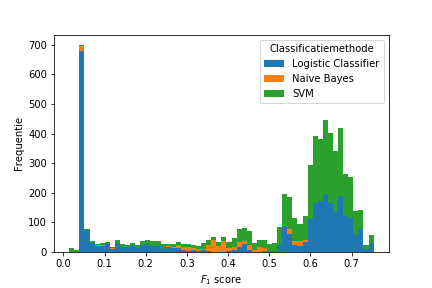
\includegraphics[width=0.50\paperwidth]{Verslag/Tables/scores.png}
\caption{Histogram van de grid search met de $F_1$ scores van de classificatiemethoden}
\label{fig:scores}
\end{figure}
Het beste resultaat werd bereikt met Support Vector Machine gebruikmakend van \textit{stochastic gradient descent learning} en L2 regularisatie. In de grid search behaalde deze methode een $F_1$ score en nauwkeurigheid van 0.75. Voor beide scores was dit het hoogste van de grid search. De woorden waren hierbij gestemd. De features waren zowel unigrams, bigrams als trigrams. Geen features zijn weggelaten door minimale of maximale documentfrequenties. De waarden van deze features waren \textit{tf-idf} scores. Het maximum aantal iteraties was 5 voor de grid search, maar de rest van resultaten zijn op basis van 100 iteraties.\par
Tabel \ref{tab:classrapport} laat de scores zien per partij met het aantal documenten in de test set. De nauwkeurigheid voor deze classificatie is 0.80. De $F_1$ scores per partij liggen tussen de 0.7 en 0.9. De partijen met een sterke focus op één onderwerp, 50PLUS, PVV en PvdD, als ook de SGP hebben hoge scores. De coalitiepartijen, VVD en PvdA, daarentegen hebben lagere scores. Figuur \ref{fig:confusionmatrix} laat zien waar de fouten in deze classificatie zitten. De meest karakteristieke n-grams per partij zijn te zien in tabel \ref{tab:MostImportantWords}. Met meest karakteristiek worden de n-grams bedoeld die de hoogste coëfficiënt hebben in de classificatie en die dus relatief het meeste belangrijk zijn voor de classificatie van een partij. Hierin is te zien dat vrijwel alle n-grams achternamen van Kamerleden of partijnamen bevatten.\par

\begin{table}[H]
\caption{Classificatie scores per partij van de beste classificatiemethode (SVM). Gemiddelde van vijfmaal kruisvalidatie.}
\label{tab:classrapport}
\centering
\begin{tabular}{lrrrlr}
\toprule
{} &  Precision &  Recall &  F1\_score & Accuracy &  Documenten \\
\midrule
50PLUS       &       0.97 &    0.85 &      0.91 &        - &        71.4 \\
CDA          &       0.80 &    0.79 &      0.80 &        - &       379.6 \\
ChristenUnie &       0.83 &    0.76 &      0.79 &        - &       215.4 \\
D66          &       0.78 &    0.75 &      0.76 &        - &       381.8 \\
GroenLinks   &       0.89 &    0.73 &      0.80 &        - &       209.2 \\
PVV          &       0.82 &    0.88 &      0.85 &        - &       345.0 \\
PvdA         &       0.72 &    0.71 &      0.71 &        - &       377.4 \\
PvdD         &       0.86 &    0.87 &      0.86 &        - &        81.2 \\
SGP          &       0.87 &    0.84 &      0.86 &        - &       134.8 \\
SP           &       0.73 &    0.85 &      0.78 &        - &       453.2 \\
VVD          &       0.77 &    0.73 &      0.75 &        - &       331.0 \\
Totaal       &       0.79 &    0.79 &      0.79 &     0.79 &      2980.0 \\
\bottomrule
\end{tabular}

\end{table}


\begin{figure}[H]
  \centering
    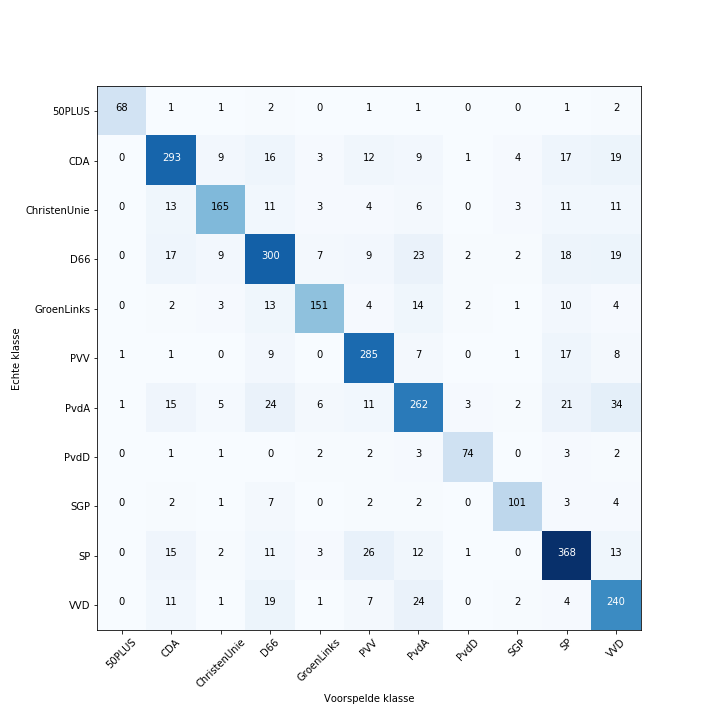
\includegraphics[width=0.50\paperwidth]{Verslag/Tables/confusionmatrix.png}
\caption{Confusion matrix van de beste classificatiemethode (SVM). Gemiddelde van vijfmaal kruisvalidatie.}
\label{fig:confusionmatrix}
\end{figure}



\begin{table}[H]
\caption{Meest karakteristieke n-grams per partij op basis van de beste classificatiemethode (SVM) gedurende kabinet-Rutte II. N-grams die niet achternamen van Kamerleden of partijnamen bevatten, zijn dikgedrukt. }
\label{tab:MostImportantWords} 
\centering
\hspace*{-1in}
\begin{tabular}{lllll}
\toprule
          50PLUS &               CDA &         ChristenUnie &                  D66 &          GroenLinks \\
\midrule
          50plus &               cda &      de christenunie &                  d66 &          groenlinks \\
   lid krol naar &           het cda &         christenunie &         mijn fractie &    lid van tongeren \\
    het lid krol &            de cda &        lid dik faber &  leden van veldhoven &   lid voortman naar \\
        lid krol &       cda fractie &          het lid dik &       lid van meenen &    het lid voortman \\
   krol naar mij &    de cda fractie &              lid dik &        van veldhoven &        lid voortman \\
       krol naar &       lid omtzigt &            dik faber &            veldhoven &            voortman \\
            krol &   het lid omtzigt &                faber &    lid van veldhoven &            tongeren \\
      van 50plus &  lid omtzigt naar &     leden voordewind &         leden schouw &        van tongeren \\
 gepensioneerden &      omtzigt naar &  de leden voordewind &      de leden schouw &  leden van tongeren \\
         ouderen &  omtzigt naar mij &                  dik &               d66 is &   de leden voortman \\
\bottomrule
\end{tabular}
 
\end{table} 
\addtocounter{table}{-1} 
\begin{table}[H]
\caption{Meest karakteristieke n-grams per partij op basis van de beste classificatiemethode (SVM) gedurende kabinet-Rutte II. N-grams die niet achternamen van Kamerleden of partijnamen bevatten, zijn dikgedrukt.  \emph{(Vervolg)}} 
\centering
\hspace*{-1.3in}
\begin{tabular}{llllll}
\toprule
              PVV &             PvdA &              PvdD &              SGP &             SP &             VVD \\
\midrule
              pvv &          de pvda &      lid ouwehand &              sgp &             sp &          de vvd \\
           de pvv &             pvda &  lid ouwehand nar &           de sgp &          de sp &             vvd \\
      islamitisch &    de partij van &  het lid ouwehand &      sgp fractie &   lid van gerv &  de vvd fractie \\
        lid graus &    van de arbeid &      ouwehand nar &   de sgp fractie &     sp fractie &     vvd fractie \\
    het lid graus &        de arbeid &  ouwehand nar mij &     led dijkgraf &  de sp fractie &       de vvd is \\
    lid graus nar &    partij van de &          ouwehand &  de led dijkgraf &   van gerv nar &          vvd is \\
          miljard &       partij van &       vor de dier &      led van der &       gerv nar &      vor de vvd \\
    graus nar mij &     pvda fractie &           de dier &  de led bisschop &   gerv nar mij &      wat de vvd \\
        graus nar &           arbeid &              dier &     led bisschop &           gerv &     vvd betreft \\
 madlener nar mij &  de pvda fractie &     de partij vor &           sgp is &       van gerv &  de vvd betreft \\
\bottomrule
\end{tabular}
 
\end{table}

\subsection{DV2: Invloed van namen}
In tabel \ref{tab:MostImportantWords} was al te zien dat de meest karakteristieke n-grams voornamelijk achternamen van Kamerleden of partijnamen bevatten. In tabel \ref{tab:rapportonlynames} zijn de scores te zien voor een classificatie met alleen achternamen van Kamerleden en partijnamen. De nauwkeurigheid is 0.61. De scores zijn gedaald ten opzichte van de resultaten van deelvraag 1, maar hoger dan de baseline scores.\par
\begin{table}[H]
\caption{Classificatierapport van beste classificatie met alleen achternamen van Kamerleden en partijnamen. Hiervoor is alleen gebruikgemaakt van unigrams. Gemiddelde van vijfmaal kruisvalidatie.}
\label{tab:rapportonlynames}
\centering
\begin{tabular}{lrrr}
\toprule
{} &  Precisie &  Sensitiviteit &  $F_1$ score \\
\midrule
50PLUS       &       0.82 &    0.88 &      0.85\\
PvdD         &       0.68 &    0.78 &      0.69 \\
GroenLinks   &       0.71 &    0.66 &      0.68  \\
PVV          &       0.66 &    0.71 &      0.67  \\
CDA          &       0.67 &    0.65 &      0.66  \\
ChristenUnie &       0.66 &    0.58 &      0.62 \\
SP           &       0.61 &    0.64 &      0.62  \\
VVD          &       0.68 &    0.57 &      0.62  \\
SGP          &       0.69 &    0.54 &      0.60  \\
D66          &       0.56 &    0.53 &      0.54  \\
PvdA         &       0.56 &    0.51 &      0.52  \\
\midrule
Totaal       &       0.64 &    0.62 &      0.62  \\
\bottomrule
\end{tabular}

\end{table}

In tabel \ref{tab:rapportwithoutnames} zijn de $F_1$ scores te zien van classificatie met achternamen van Kamerleden en partijnamen vervangen. De nauwkeurigheid hiervan is 0.58. De scores zijn lager dan die uit deelvraag 1 en lager dan van de classificatie met alleen namen. Wel zijn de scores nog steeds hoger dan de baseline. In tabel \ref{tab:MostImportantWordsWithoutNames} is vervolgens te zien welke n-grams het meest karakteristiek zijn per partij voor deze classificatie.\par
\begin{table}[H]
\caption{Classificatie scores per partij van beste classificatiemethode (SVM) uit deelvraag 1 zonder achternamen van Kamerleden en partijnamen met het relatieve verschil in $F_1$ score ten opzichte van tabel \ref{tab:classrapport}. Gemiddelde van vijfmaal kruisvalidatie.}
\label{tab:rapportwithoutnames}
\centering
\begin{tabular}{lcccc}
\toprule
{} &  Precision &  Recall &  $F_1$ score &  $\Delta F_1$ score (\%) \\
\midrule
SGP          &       0.71 &    0.73 &      0.72 & -18 \\
PvdD         &       0.75 &    0.70 &      0.72 & -19 \\
PVV          &       0.63 &    0.80 &      0.70 & -19 \\
ChristenUnie &       0.68 &    0.46 &      0.55 & -21 \\
CDA          &       0.52 &    0.53 &      0.52 & -23 \\
SP           &       0.54 &    0.71 &      0.61 & -24 \\
D66          &       0.55 &    0.55 &      0.55 & -28 \\
VVD          &       0.54 &    0.49 &      0.52 & -30 \\
50PLUS       &       0.86 &    0.49 &      0.62 & -32 \\
PvdA         &       0.51 &    0.48 &      0.50 & -32 \\
GroenLinks   &       0.64 &    0.38 &      0.48 & -41 \\
\midrule
Totaal       &       0.59 &    0.58 &      0.57 &        -29 \\
\bottomrule
\end{tabular}

\end{table}

\begin{table}[H] 
\caption{Meest karakteristieke n-grams per partij op basis van de classificatiemethode (SVM) uit deelvraag 1 zonder achternamen van Kamerleden en partijnamen gedurende kabinet-Rutte II.} 
\label{tab:MostImportantWordsWithoutNames} 
\centering
\hspace*{-0.8in}
\begin{tabular}{lllll}
\toprule
                 50PLUS &             CDA &   ChristenUnie &           D66 &              GroenLinks \\
\midrule
        gepensioneerden &  PARTIJ fractie &   mensenhandel &  mijn fractie &                     zou \\
                ouderen &        inwoners &         zullen &          mijn &       kamer hierover te \\
                 oudere &          PARTIJ &       gezinnen &       fractie &     belastingontwijking \\
 koopkrachtontwikkeling &        regering &      inderdaad &    natuurlijk &            in elk geval \\
               plussers &             wij &  vluchtelingen &   het kabinet &        persoonsgebonden \\
                     50 &     de regering &       kinderen &    belangrijk &               elk geval \\
              werkenden &            hier &           hoop &       vandaag &                  in elk \\
            50 plussers &            echt &          motie &        kansen &  hierover te informeren \\
   voor gepensioneerden &         fractie &     onder meer &       kabinet &          schone energie \\
            overwegende &              de &     constateer &  buitengewoon &             hierover te \\
\bottomrule
\end{tabular}
 
\end{table} 
\addtocounter{table}{-1} 
\begin{table}[H] 
\caption{Meest karakteristieke n-grams per partij op basis van de classificatiemethode (SVM) uit deelvraag 1 zonder achternamen van Kamerleden en partijnamen gedurende kabinet-Rutte II. \emph{(Vervolg)}} 
\centering
\hspace*{-1.3in}
\begin{tabular}{llllll}
\toprule
         PVV &             PvdA &              PvdD &                    SGP &            SP &            VVD \\
\midrule
 islamitisch &      mijn partij &              dier &               dank zer &       huurder &     volgen mij \\
       islam &       leerkracht &            de bio &  mevrouw de voorzitter &    segregatie &        liberal \\
     miljard &           tevred &     bio industrie &             mevrouw de &      herindel &      speelveld \\
    de islam &        circulair &               bio &           eenverdiener &        armoed &     verzekerar \\
 asielzoeker &   open standaard &        aan de bio &               allerlei &     de bevolk &          aruba \\
     brussel &          gezamen &  de bio industrie &                   punt &       jazeker &     ondernemer \\
   nederland &       ieder kind &            milieu &                 nadruk &          zegt &       regelgev \\
       grenz &  duurzam energie &     dierenwelzijn &                  woord &  bureaucratie &       aangegev \\
  immigratie &               en &          de natur &                 vanuit &     tenderned &  PARTIJNAAM is \\
          al &       lager over &   klimaatverander &                    oog &  ouderbijdrag &     essentieel \\
\bottomrule
\end{tabular}
 
\end{table}



\subsection{DV3: Oppositie of regering}
In figuur \ref{fig:distributies} zijn de distributies van de errors, zoals gedefinieerd in formule \ref{eq:error} te zien van combinaties van regerings- en oppositiepartijen. Bijgevoegd zijn het aantal combinaties (N), het gemiddelde ($\mu$) en de standaarddeviatie ($\sigma$).
\begin{figure}[H]
    \centering
    \hspace*{-0.2in}
    \subfloat[Tussen twee regeringspartijen (N=200, \protect\\Mediaan=25.83, IKA=9.18)]{{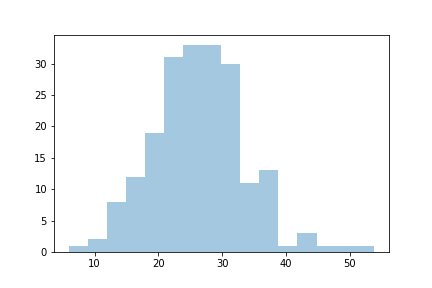
\includegraphics[width=7cm]{Verslag/Handmatig/Regering.png} }}%
    \subfloat[Tussen twee oppositiepartijen (N=8100, \protect\\Mediaan=-1.09, IKA=4.98)]{{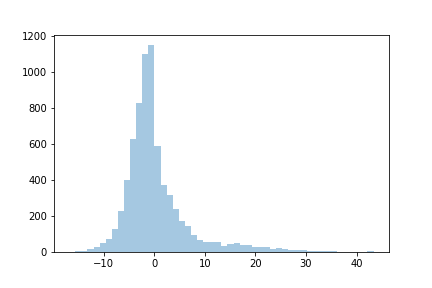
\includegraphics[width=7cm]{Verslag/Handmatig/Oppositie.png} }}\quad
    \hspace*{-0.2in}
    \subfloat[Tussen een regeringspartij en een oppositiepartij (N=4000, Mediaan=-2.92, IKA=6.82)]{{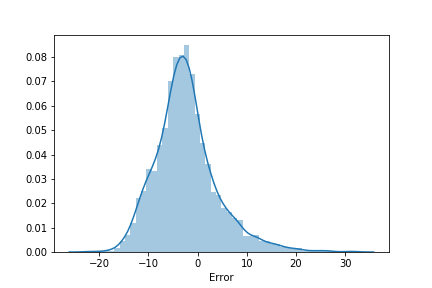
\includegraphics[width=7cm]{Verslag/Handmatig/Mix.png} }}%
    \subfloat[Totaal (N=12100, Mediaan=-1.40, IKA=5.76)]{{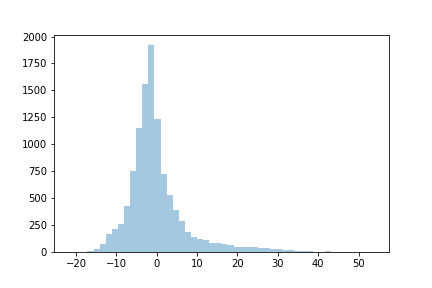
\includegraphics[width=7cm]{Verslag/Handmatig/Totaal.png} }}\quad
    \caption{Genormaliseerde distributie van de error uit formule \ref{eq:error} voor de verschillende combinaties.}%
    \label{fig:distributies}%
\end{figure}
Voor alle distributies was de nulhypothese verworpen dat deze normaal verdeeld zijn ($p < 0.01$) door middel van een normaalheidstoets. In tabel \ref{tab:whitney} is te zien dat er een significant verschil is tussen de distributies binnen regering en binnen oppositie tegenover de distributie tussen een regeringspartij en een oppositiepartij. Binnen regeringspartijen zijn er gemiddeld 26.11 misclassificaties meer dan verwacht en binnen oppositiepartijen gemiddeld 0.43.

\begin{table}[H]
\caption{Uitslagen van eenzijdige Mann-whitneytoets tussen de distributie tussen een regeringspartij en oppositiepartij en twee distributies. $\alpha$ is 0.01.}
\label{tab:whitney}
\centering
\begin{tabular}{lrr}
\toprule
{} &  $p$-waarde &  $U$-waarde\\
\midrule
Tussen twee regeringspartijen       &       \num{7.04e-124} &    717042 \\
Tussen twee oppositiepartijen         &       \num{4.4e-108} &    16328471 \\
\bottomrule
\end{tabular}
\end{table}
In tabel \ref{tab:WoordenBalkenende4} zijn de meest karakteristieke n-grams te zien voor classificatie van kabinet-Balkenende IV. Hierin zijn geen opvallende overlappen te zien van regeringspartijen met de classificatie van kabinet-Rutte II in tabel \ref{tab:MostImportantWordsWithoutNames}.
\begin{table}[H] 
\caption{Meest karakteristieke n-grams per partij op basis van beste classificatiemethode uit deelvraag 1 zonder achternamen van Kamerleden en partijnamen gedurende kabinet-Balkenende IV.} 
\label{tab:WoordenBalkenende4} 
\centering
\hspace*{-0.6in}
\begin{tabular}{lllll}
\toprule
                  CDA &        ChristenUnie &              D66 &          GroenLinks &         PVV \\
\midrule
       PARTIJ fractie &  fractie van PARTIJ &          premier &       PARTIJfractie &     burgers \\
                  wij &      de fractie van &       de premier &  fractie van PARTIJ &        onze \\
              fractie &          de fractie &          ik hoop &          de fractie &        niet \\
           wij hebben &         fractie van &     arbeidsmarkt &      de fractie van &        deze \\
             KAMERLID &        mijn fractie &  de arbeidsmarkt &         fractie van &  immigratie \\
                 dank &             geweest &             hoop &           politieke &  natuurlijk \\
 PARTIJ fractie heeft &              moment &              hij &             premier &     politie \\
          zorgvuldige &             termijn &   schone energie &                deal &  de burgers \\
                  ons &       verschillende &          plannen &                  ik &      burger \\
         buitengewoon &       beantwoording &           kunnen &                  en &        door \\
\bottomrule
\end{tabular}
 
\end{table} 
\addtocounter{table}{-1} 
\begin{table}[H] 
\caption{Meest karakteristieke n-grams per partij op basis van beste classificatiemethode uit deelvraag 1 zonder achternamen van Kamerleden en partijnamen gedurende kabinet-Balkenende IV.\emph{(Vervolg)}} 
\centering
\hspace*{-0.4in}
\begin{tabular}{lllll}
\toprule
         PvdA &              PvdD &                    SGP &            SP &             VVD \\
\midrule
          wij &            dieren &           mijn fractie &          zegt &          PARTIJ \\
   belangrijk &     dierenwelzijn &          beantwoording &    leerlingen &    onze fractie \\
      vrouwen &     bio industrie &                    wel &        mensen &  PARTIJ fractie \\
         alle &            natuur &          de voorzitter &            is &         fractie \\
          ben &  de bio industrie &       de voorzitter ik &          niet &              je \\
  volgens mij &            de bio &             natuurlijk &       vandaar &     ondernemers \\
           of &               bio &                diverse &  bureaucratie &            awbz \\
 mijn collega &       dierproeven &               allerlei &            nu &           markt \\
   antwoorden &       veehouderij &      voorzitter ik wil &   voorstellen &          praten \\
         punt &         industrie &  mevrouw de voorzitter &       leraren &      timmermans \\
\bottomrule
\end{tabular}
 
\end{table}
In tabel \ref{RegeringOppositie} zijn de scores te zien van de classificatie die getraind is op een zittingsperiode, maar getest op een andere. De resultaten zijn gedaald, maar nog boven de baseline. De daling verschilt per partij en zittingsperiode met dalingen van $F_1$ scores tussen 12 en 92\%. \par
\begin{table}[H]
\caption{$F_1$ scores van de classificatie getraind op de dataset van Balkenende IV of Rutte II (minus 50PLUS) en getest op de ander. Scores van een classificatie getraind en getest op kabinet-Rutte II zonder 50PLUS zijn bijgevoegd ter referentie, als ook de relatieve daling. De classificatiemethode uit deelvraag 1 is gebruikt zonder achternamen van Kamerleden en partijnamen. Partijen met een asterisk zijn gewisseld van partij-status.}
\centering
\hspace*{-0.2in}
\label{RegeringOppositie}
\begin{tabular}{ll|cccc}
\toprule
{}& {}&\multicolumn{4}{l}{Training set$\rightarrow$ Test set}\\
\midrule
{} &Rutte II &\multicolumn{2}{l}{\makecell{Balkenende IV $\rightarrow$ Rutte II\\Baseline = 0.11}}&  \multicolumn{2}{l}{\makecell{Rutte II $\rightarrow$ Balkenende IV\\Baseline = 0.12}}  \\
{} & $F_1$ & $F_1$ & $\Delta F_1$ score (\%) &  $F_1$& $\Delta F_1$ score (\%) \\
\midrule
SGP          &0.74&       0.56 &  -24 &   0.49 & -34 \\
PvdD         &0.73&       0.64 &  -12 &  0.45 & -38\\
PVV          &0.70&       0.50 &  -29 &   0.60  & -14 \\
SP           &0.61&       0.41 & -33 &   0.53 & -13 \\
ChristenUnie* &0.55&       0.37 &  -33 & 0.22 &-60 \\
D66          &0.54&       0.16 &  -70 & 0.28 & -48 \\
CDA*          &0.53&       0.28 & -47&   0.43 & -19 \\
PvdA         &0.52&       0.29 & -44 &   0.27 & -48 \\
VVD*          &0.51&       0.18 & -65 &   0.10 & -80  \\ 
GroenLinks   &0.49&       0.31 &  -37 &   0.04 & -92 \\ \hline
Totaal       &0.58&       0.34 & -41 &  0.35 & -40 \\
\bottomrule
\end{tabular}

\end{table}


\subsection{DV4: Links-rechts as}
In tabel \ref{fig:distanceerror} is de error te zien ten opzichte van de afstand op de links-rechts as.
\begin{figure}[H]
  \centering
    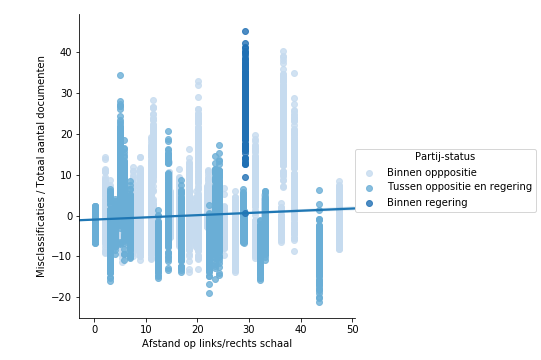
\includegraphics[width=0.60\paperwidth]{Verslag/Tables/Ideology.png}
\caption{Error ten opzichte van de afstand op de links-rechts as van twee partijen. Gebaseerd op 100 classificaties met verschillende test en train set. De Pearson correlatie is 0.09 en de $p$-waarde \num{2.39e-20}.}
\label{fig:distanceerror}
\end{figure}
De Pearson correlatie van 0.09 is daarmee met een $p$-waarde van \num{2.39e-20} significant op het significantieniveau van 0.01, maar wel positief gecorreleerd. Uit deelvraag 3 bleek dat de error binnen oppositie of regering significant afweek van de error tussen regering en oppositie. Dit effect lijkt ook zichtbaar in figuur \ref{fig:distanceerror}. Daarom is er ook gekeken naar de correlatie tussen afstand op de links-rechts as en error binnen oppositie en tussen regerings- en oppositiepartij. De resultaten zijn te zien in tabel \ref{tab:pearson}. Beide correlaties zijn statistische significant op het significantieniveau van 0.01, maar in tegengestelde richting.

\begin{table}[H]
\caption{Pearson correlatie tussen error en afstand op de links-rechts as voor combinaties van partij-status.}
\label{tab:pearson}
\centering
\begin{tabular}{lrr}
\toprule
{} &  Pearson correlatie &  $p$-waarde\\
\midrule
Tussen oppositie- en regeringspartij       &       -0.29 &    \num{3.44e-69} \\
Tussen twee oppositiepartijen         &       0.18 &    \num{1.76e-55} \\
\bottomrule
\end{tabular}
\end{table}

\subsection{DV5: Woordgebruik van sprekers}
In tabel \ref{tab:rapporttaalgebruik} staan de scores van classificatie waarbij de Kamerleden verdeeld zijn over de training en test set. De scores zijn hierbij nauwelijks hoger dan de baseline.
\begin{table}[H]
\caption{Classificatierapport van beste classificatiemethode uit deelvraag 1 zonder achternamen van Kamerleden en partijnamen met de Kamerleden verdeeld over training en test set. Gemiddelde van tienmaal kruisvalidatie.}
\label{tab:rapporttaalgebruik}
\centering
\begin{tabular}{lrrrr}
\toprule
{} &  Precisie &  Sensitiviteit &  $F_1$ score &  $\Delta F_1$ score (\%) \\
\midrule
50PLUS       &       0.29 &    0.06 &      0.09 &           \\
CDA          &       0.12 &    0.20 &      0.14 &          \\
ChristenUnie &       0.08 &    0.14 &      0.09 &           \\
D66          &       0.22 &    0.22 &      0.22 &          \\
GroenLinks   &       0.16 &    0.04 &      0.05 &          \\
PVV          &       0.29 &    0.50 &      0.37 &          \\
PvdA         &       0.25 &    0.19 &      0.21 &          \\
PvdD         &       0.46 &    0.17 &      0.22 &          \\
SGP          &       0.17 &    0.05 &      0.07 &           \\
SP           &       0.34 &    0.33 &      0.33 &          \\
VVD          &       0.31 &    0.26 &      0.24 &          \\
\midrule
Totaal       &       0.31 &    0.24 &      0.24 &         \\
\bottomrule
\end{tabular}

\end{table}


\section{Conclusions}
\label{sec:conc}

Hierin beantwoord je jouw hoofdvraag op basis van het eerder vergaarde bewijs.



\subsection{Acknowledgements}
Hier kan je bedanken wie je maar wilt.

% your refs

\bibliographystyle{plain}
\bibliography{MyThesis}

\appendix

%\input{appendix}


\section{Slides}

% Example
\includepdf[nup=2x3 , pages=-]{sargent-lecture_slides.pdf}
 
\end{document}
